\noindent
Microfluidic T-junctions are used for creating dispersed bubbles or droplets
of a consistent volume. Such platforms have been used for a variety of applications,
such as chemical microreactors, biological screening assays, and DNA analysis.
It is often critical that the volume of the
bubbles or droplets are consistent and predictable. A mathematical model was
previously developed by van Steijn \emph{et al.,} for predicting the volume of bubbles and droplets formed in
microfluidic T-junctions, however, their code was not made readily available.
In this work, we develop Python modules that implement the mathematical model and 
replicate the figures in the original work. The model
could be fully replicated based solely on the contents of the original article.
However, one figure provided in the original work was inconsistent with the
model equations while another could be replicated but with a small discrepancy.

\section{Introduction}

\subsection{Microfluidic T-junctions}

Microfluidic T-junctions are microfluidic devices composed of T-shaped junctions
where cross-flowing streams occur. Droplet formation in microfluidic T-junction
occurs at the junction where liquid or gas from the side channel (dispersed phase)
meets with liquid in the main channel (continuous phase). The dispersed phase forms
a plug shape due to the shear and extrusion of the continuous phase and rupture due
to the instability of interface\supercite{huang_precise_2020}. The size of the
resulting droplets heavily relies on the channel geometry, flow rate ratio, and device
surface properties\supercite{dreyfus_ordered_2003}. Microfluidic T-junctions have been
applied in biological, chemical, and biomedical
fields\supercite{casadevall_i_solvas_droplet_2011}.
For example, chemical microreactors that allow very small-scale chemical reactions, high
throughput biological screening assays, and DNA analysis\supercite{ibrahim_modeling_2021}.
The ability to precisely predict the size of bubbles and droplet generated in microfluidic
T-junctions is very important because many of these applications require
precise sample volume as determined by droplet size.

\subsection{Models for size prediction}

Since several parameters can affect droplet formation in microfluidic T-junctions, it
can be difficult to precisely tune the droplet size \emph{a priori}. Many models
have been reported to solve this issue. For example, a numerical simulation approach was proposed, utilizing a
hydrodynamic model to predict droplet size by varying capillary numbers,
flow rate ratios, viscosity ratios, and contact angles\supercite{liu_droplet_2009}.
In a study by Steegmans \emph{et al.,} a statistical model based on the data from
experiments in other published works was developed to model droplet break-up in T-junctions. Their approach divided
the process into two phases: (1) droplet growth, and (2) detachment phase\supercite{steegmans_generalised_2009}.
Another study concluded that the effects of surface force and viscous force dominate
the droplet stream generated in their microfluidic T-junction system based on numerical
results, theoretical analysis, and experimental measurements\supercite{li_study_2012}.
A volume-of-fluid model was introduced to investigate the droplet formation process
by varying the dispersed phase flow rate under a constant capillary
number\supercite{soh_numerical_2016}. 

In this work, we aim to replicate the mathematical model based on
geometrical parameters to predict the size of bubbles (liquid continuous phase, gas dispersed phase)
and droplets (liquid in both continuous and dispersed phase) created in
microfluidic T-junctions published by van Steijn \emph{et al.,}\supercite{van_steijn_predictive_2010}
which was consistent with the model presented by Steegmans \emph{et al.}

\subsection{van Steijn et al. model overview}

The model presented in the original work by van Steijn \emph{et al.}
divides the droplet formation process into two phases: \emph{filling} and \emph{squeezing}. The final model
adds the contributions from the two stages to arrive at the droplet/bubble volume.
This is summarized as the dimensionless volume in the following equation:

\begin{equation}
  \frac{V}{hw^2} = \frac{V_{fill}}{hw^{2}}+\alpha\frac{q_{d}}{q_{c}}
\end{equation}

\subsubsection{Filling phase}

The filling phase begins as the dispersed fluid enters the main
channel from the inlet channel. This phase continues until the emerging
dispersed fluid reaches the far side of the main channel, at which time
the squeezing phase begins.

The equation describing the filling phase defines the dimensionless fill volume as:

\begin{equation}
  \frac{V_{fill}}{hw^{2}} = 
    \begin{cases}
      \frac{3\pi}{8} - \frac{\pi}{2} \left(1 - \frac{\pi}{4}\right) \frac{h}{w} & \quad \text{for } w_{in} \leq w\\
      \left(\frac{\pi}{4} - \frac{1}{2} \arcsin\left(1-\frac{w}{w_{in}}\right)\right) \left(\frac{w_{in}}{w}\right)^2 + \\
      -\frac{1}{2} \left(\frac{w_{in}}{w} - 1\right) \left(2\frac{w_{in}}{w} - 1\right)^\frac{1}{2} +
      \frac{\pi}{8} + \\
      -\frac{1}{2} \left(1 - \frac{\pi}{4}\right) \left(\left(\frac{\pi}{2} - \arcsin\left(1 - \frac{w}{w_{in}}\right)\right)\frac{w_{in}}{w} + \frac{\pi}{2}\right)\frac{h}{w}
      & \quad \text{for } w_{in} > w
    \end{cases}\label{nondim_fill_vol}
\end{equation}

\noindent This equation is derived strictly based on geometries that are present when the
emerging dispersed phase reaches the far wall of the main channel.

\subsubsection{Squeezing phase}

Once the dispersed phase reaches the far wall of the main channel, the squeezing
phase begins. The contribution to the total dimensionless volume during the
squeezing phase is described by the following equation:

\begin{equation}
  \frac{V_{squeeze}}{hw^2} = {\alpha}\frac{q_d}{q_c}\label{nondim_squeeze_vol}
\end{equation}

\noindent The squeezing coefficient ($\alpha$) is described by Equation \eqref{alpha}:

\begin{equation}
  \alpha = \left(1 - \frac{\pi}{4}\right)
  \left(1 - \frac{q_{gutter}}{q_{c}}\right)^{-1}
  \left(\left(\frac{R_{pinch}}{w}\right)^2 -
  \left(\frac{R_{fill}}{w}\right)^2 +
  \frac{\pi}{4}\left(\frac{R_{pinch}}{w} -
  \frac{R_{fill}}{w}\right)\frac{h}{w}\right)\label{alpha}
\end{equation}

\noindent Where the radius denoted $R_{fill}$ is determined by:

\begin{equation}
  R_{fill} = \max\left(w,w_{in}\right)\label{R_fill}
\end{equation}

\noindent And the radius denoted $R_{pinch}$ is described by:

\begin{equation}
  R_{pinch} = w + w_{in} - \left(\frac{hw}{h+w} - \varepsilon\right) +
  \left(2\left(w_{in} -
    \left(\frac{hw}{h+w} -
    \varepsilon\right)\right)\left(w -
    \left(\frac{hw}{h+w} - \varepsilon\right)\right)\right)^\frac{1}{2}\label{R_pinch}
\end{equation}

\noindent The original authors determined experimentally that $\frac{q_{gutter}}{q_c}=0.1$,
so this relationship is used during all calculations in the original work.

\section{Methods}

All code used for replication was written in Python\supercite{pypi_python_nodate}
v3.11.0 and using the conda\supercite{noauthor_conda_2017} package manager v22.9.0.
Code was developed using Windows Subsystem for Linux 2 (WSL2)\supercite{microsoft_windows_nodate}
connected to an Ubuntu\supercite{canonical_ltd_ubuntu_2020} v20.04 kernel.

\subsection{Python modules}

Three Python modules were developed which capture the model logic allowing for the prediction of
bubble/droplet size prediction. The modules are divided into the filling phase and squeezing phase,
and a third module can be used to calculate the total predicted volume by combining the contributions
of those two phases.

\subsubsection{Filling phase}

While dimensionless fill volume could be calculated directly using equation \eqref{nondim_fill_vol},
we took a more verbose approach in developing the filling module. This is to aid in readability and
interpretability of the functions defined in the module.

We begin with the provided definition of fill volume ($V_{fill}$) as the gross volume
($V_{gross}$) minus the total gutter volume ($2V_{gutter}$).

$V_{gross}$ is calculated as the cross-sectional area of the emerging droplet ($A_{droplet}$)
at the midplane extruded by the channel height ($h$).

$V_{gutter}$ is calculated as cross sectional area of the gutter ($A_{gutter}$) extruded along
the perimeter of the emerging droplet ($l_{gutter}$).

This is summarized as:

\begin{equation}
  V_{fill} = V_{gross} - 2V_{gutter} = hA_{droplet} - 2A_{gutter}l_{gutter} \label{fill_vol}
\end{equation}

\noindent In the module, $A_{droplet}$ is calculated piece-wise using geometry (\emph{e.g.} area of quarter circle with 
radius $w$ plus area of half circle with radius $\frac{w}{2}$). A simplified version of this is given by:

$$
A_{droplet} = 
    \begin{cases}
      \frac{3\pi}{8}w^2 & \quad \text{for } w_{in} \leq w\\
      \frac{\pi}{8}w^2 + \frac{\pi}{4}w_{in}^2 \\
      - w_{in}^2\frac{1}{2}\arcsin{\left(\frac{w_{in}-w}{w_{in}}\right)} \\
      - \frac{1}{2}\left(w_{in}-w\right)\sqrt{w_{in}^2 - \left(w_{in}-w\right)^2} & \quad \text{for } w_{in} > w
    \end{cases}
$$

\noindent Similarly, $l_{gutter}$ is calculated using basic geometric shapes, and a simplified
equation is given by:

$$
l_{gutter} = 
    \begin{cases}
      {\pi}w & \quad \text{for } w_{in} \leq w\\
      \frac{\pi}{2}w+w_{in}\left(\frac{\pi}{2}-\arcsin\left(1-\frac{w}{w_{in}}\right)\right) & \quad \text{for } w_{in} > w
    \end{cases}
$$


\noindent The simplified equation for the cross-sectional area of the gutter is:
$$A_{gutter} = \frac{8-\pi}{16}h^2$$

\noindent The module calculates the fill volume by individually calculating the variables in equation
\eqref{fill_vol} using the described relationships.
This is then divided by $hw^2$ to make it non-dimensionalized.

To ensure that the verbose geometric implementation matches the simplified equation \eqref{nondim_fill_vol}, 
unit tests compare the values obtained using each version.

\subsubsection{Squeezing phase}
The non-dimensionalized volume during the squeezing period is given by equation \eqref{nondim_squeeze_vol}, with
equations for the variables defined in equations \eqref{alpha}, \eqref{R_fill}, and \eqref{R_pinch}.

Functions for calculating each of the intermediate variables and non-dimensionalized squeeze volume
were developed, each with accompanying unit tests.

\subsection{Replication of figures}

To fully replicate the results in the original work, the figures showing model outputs were
replicated using the modules that were developed. A Python script imports the necessary
functions from the modules and uses Pandas\supercite{team_pandas_2020} v1.5.1
and plotnine\supercite{kibirige_plotnine_2022} v0.10.1 to create the figures.
This section will describe how each figure was replicated.

For convenience in discussing the figures of the original work, we will prepend figure names
with “O” to distinguish them from the figures presented in this manuscript. For example, Figure 2 from
the original work will be referred to as Figure O2.

Figure O2 has two panels, which are unlabeled in the original work. We will refer to these as Figure O2a
(left panel) and Figure O2b (right panel) for convenience.

\subsubsection{Figure O2a}

Figure O2a shows the non-dimensionalized volume during the filling phase ($\frac{V_{fill}}{hw^2}$)
against the ratio of channel height over channel width ($\frac{h}{w}$) for four width ratios 
($\frac{w_{in}}{w}$).
To replicate this figure, a series of 1000 data points were generated spanning $\frac{h}{w} \in [0,0.5]$
for each $\frac{w_{in}}{w}$, arbitrarily setting $w=1$, and varying $h$ and
$w_{in}$ to obtain the necessary ratios.

The dimensionless fill volume was then calculated for each point using the module that was
developed. These series of points were then plotted, the axes were scaled identically to the
original work.

\subsubsection{Figure O2b}

Figure O2b shows the squeezing coefficient ($\alpha$) against the same range of $\frac{h}{w}$
values as Figure O2a. However, six width ratios ($\frac{w_{in}}{w}$) are plotted.

This figure was again replicated using 1000 data points per width ratio. Channel width ($w$) was
held constant while $h$ and $w_{in}$ were varied. As in the original work the corner roundness
$\varepsilon=0$. The flow rate of the continuous phase was set as $q_c=1$, and the flow rate of the
gutter was calculated as $q_{gutter}=0.1*q_c$ such that $\frac{q_{gutter}}{q_c}=0.1$, as described
in the original work.

The squeezing coefficient was calculated based on these values using the function in the
squeezing module, and plotted using the same axis scales as the original work.

\subsubsection{Figure O3}

Figure O3 shows the dimensionless volume of droplets and bubbles against the flow rate ratio
of the dispersed phase over the continuous phase ($\frac{q_d}{q_c}$). Six series are plotted,
five are air bubbles produced using five width ratios ($\frac{w_{in}}{w}$) and varying heigth over width
values ($\frac{h}{w}$); the final series shows liquid-liquid droplets with $\frac{w_{in}}{w} = 1$ and
$\frac{h}{w}=0.48$. For air bubbles $\varepsilon=0.1w$ and for liquid-liquid droplets $\varepsilon=0.01w$.

For replication, continuous flow rate ($q_c$) and channel width ($w$) were both set equal to $1$.
Channel height ($h$), inlet width ($w_{in}$), and dispersed phase flow rate ($q_d$) were all varied to
achieve the necessary ratios. Corner roundness ($\varepsilon$) was computed based on channel width using the
relationship described above. 1000 data points were generated for each of the six series.

The total dimensionless volume was calculated using the module that combines the squeezing and filling
phase contributions. This total dimensionless volume was plotted
in the same manner as in the original work.

\subsubsection{Figure O6}

Figure O6 shows the shortest distance between the receding interface from the channel wall ($2r$) normalized
by channel width ($2r/w$) against time ($t$) multiplied by $\frac{q_c}{hw^2}$. Where continuous phase
flow rate $q_c = 3{\mu}L\;\mathrm{min}^{-1}$, height $h=33{\mu}m$, width $w=100{\mu}m$, and corner roundness
$\varepsilon=0.1w$. Three series are shown, corresponding to various width ratios ($\frac{w_{in}}{w}$).
Additionally, a horizontal line, $\frac{2r_{pinch}}{w}=\frac{h}{h+w}$, is added corresponding to
the predicted threshold at which pinch-off of the droplet occurs.

While the independent axis ($\frac{q_c}{hw^2}t$) can be generated using the provided geometries, and varying
time to get values in the required range (\emph{i.e.,} $\frac{q_c}{hw^2}t \in [0,10]$), the dependent axis,
$2r/w$ must computed as a function of $\frac{q_c}{hw^2}t$. Since $\frac{q_c}{hw^2}$ and $w$ are all constant,
this amounts to needing $2r$ as a function of $t$. Although no such equation
is explicitly provided in the original work, it can be inferred.

To do so, the relationship between $2r$ and $R$, which is given in the original work, will be used:

\begin{equation}
  2r - \varepsilon = R - \sqrt{\left(R - w\right)^2 + \left(R - w_{in}\right)^2}
\end{equation}

\noindent But first, an equation must be found that gives $R$ as a function of time. The equation
relating $R$ and $t$ is given by:

\begin{equation}
  \left[2\frac{R}{w} + \frac{\pi}{4}\frac{h}{w}\right]
  \frac{\mathrm{d}}{\mathrm{d}t}\left(\frac{R}{w}\right) = 
  \frac{q_c}{hw^2} \left(1-\frac{\pi}{4}\right)^{-1}
  \left(1-\frac{q_{gutter}}{q_c}\right)
\end{equation}

\noindent Multiplying both sides by $w^2$ and integrating with respect to $\mathrm{d}t$:

$$
  \int_{0}^t{\left[2R + \frac{h\pi}{4}\right]
  \frac{\mathrm{d}R}{\mathrm{d}t}} \mathrm{d}t = 
  \int_{0}^t{\frac{q_c}{h} \left(1-\frac{\pi}{4}\right)^{-1}
  \left(1-\frac{q_{gutter}}{q_c}\right)} \mathrm{d}t
$$

\noindent Evaluating the integrals:

$$ 
  \left. R^2 + \frac{h\pi}{4}R \right|_{t=0}^{t}=
  \left. \frac{q_c}{h}
  \left(1-\frac{\pi}{4}\right)^{-1}
  \left(1-\frac{q_{gutter}}{q_c}\right)t \right|_{t=0}^{t}
$$

\noindent Where $R$ is a function of time \emph{i.e.,} $R=R\left(t\right)$ and since
$t$ is taken as the time since transition from filling to squeezing,
$\left. R\left(t\right)\right|_{t=0} = R_{fill}$. Evaluating yields:

$$
  R^2 - R_{fill}^2 + \frac{h\pi}{4}\left(R-R_{fill}\right) = 
  \frac{q_c}{h}
  \left(1-\frac{\pi}{4}\right)^{-1}
  \left(1-\frac{q_{gutter}}{q_c}\right)t
$$

\noindent Setting equal to zero and rearranging:

$$
  R^2 + \frac{h\pi}{4}R -
  R_{fill}^2 - \frac{h\pi}{4}R_{fill} -
  \frac{q_c}{h}
  \left(1-\frac{\pi}{4}\right)^{-1}
  \left(1-\frac{q_{gutter}}{q_c}\right)t = 0
$$

\noindent $R$ can be solved for using the quadratic equation to yield:

\begin{equation}
  R = \frac{-\frac{h\pi}{4} \pm 
  \sqrt{\left(\frac{h\pi}{4}\right)^2 +
  4\left(R_{fill}^2 + \frac{h\pi}{4}R_{fill} +
  \frac{q_c}{h}
  \left(1-\frac{\pi}{4}\right)^{-1}
  \left(1-\frac{q_{gutter}}{q_c}\right)t\right)}}{2}
\end{equation}

\noindent Therefore $R$ can be evaluated as a function of time (taking the positive of the square root) and
$2r$ can then be calculated as:

\begin{equation}
  2r = R - \sqrt{\left(R - w\right)^2 + \left(R - w_{in}\right)^2} + \varepsilon
\end{equation}

\noindent Functions for both $R$ as a function of time, and $2r$ were added
to the squeezing module.

For replication of Figure O6, the provided geometries for $w$, $h$, and $q_c$ were used. 1000 data
points for each inlet width ratio were generated spanning $\frac{q_c}{hw^2}t \in [0,10]$ by varying 
$t$. Corner roundness ($\varepsilon$) was calculated based on $w$ as described. $2r$ was
computed using the squeezing module and divided by $w$ for plotting. As in Figure O6, linetype
was mapped to dispersed fluid type (liquid droplets vs. gas bubbles).

\subsection{Code quality}

To maintain quality of the code that was developed, several precautions were taken.

As previously mentioned, the functions developed in the modules
have associated unit tests. For the filling module, unit tests ensure that the verbose
geometric calculations match the simplified equations in the original work.
Pytest\supercite{krekel_pytest_2004} v7.2.0 testing framework was used for all unit tests.
Code coverage of the tests is assessed using coveragepy\supercite{batchelder_coveragepy_nodate} v7.1.0.
Additionally, an integration test was written for the Python script that generates the
replicated figures, ensuring that it can be run and generate figures as output.

Black\supercite{langa_black_2018} v23.1.0 was used to format all Python files. 
Several static code checks were employed to automatically assess code quality.
Pylint\supercite{thenault_pylint_2001} v2.15.5 and
Flake8\supercite{ziade_flake8_2011} v5.0.4 were used for static code checking
and linting, which adhere to PEP8\supercite{van_rossum_pep_2001} standards. Type annotations were employed
in all Python code, and mypy\supercite{lehtosalo_mypy_2012} v0.990 was used for
static type checking.

A Make\supercite{feldman_gnu_1988} v4.2.1 target was added to perform automatic execution of all
unit tests and static code checks with a single command.

\section{Results}

\subsection{Python modules}

Three Python modules were developed implementing the model presented in the original work.

The filling module consists of 8 functions and 8 unit tests. The squeezing module consists
of 8 functions and 7 unit tests. Finally, the module combining the two phases of droplet formation
consists of  2 functions and 2 unit tests. All modules have 100\% test coverage as evaluated by
coveragepy. All code passes static checking by Pylint, Flake8, and mypy.

\subsection{Replication of figures}

All figures showing modeling results in the original work were replicated. 

\subsubsection{Figure O2a}

The figure generated using our modules (Figure \ref{fig2a}) is similar to
Figure O2a in the original work. However, for $\frac{w_{in}}{w}>1$, the
lines have a markedly more negative slope than those in Figure O2a.

Interestingly however, a plot matching Figure O2a could be achieved
(Figure \ref{fig2a_bad}). To do so,
a separate function was written to calculate the dimensionless fill volume. In this function,
the volume is not calculated using geometry, but instead uses the equation in the original work,
but neglecting a pair of parentheses.

The portion of equation \eqref{nondim_fill_vol} that was modified is as follows.
The equation presented in the original work contains:

$$
\left(\left(\frac{\pi}{2} -
\arcsin\left(1 - \frac{w}{w_{in}}\right)\right)\frac{w_{in}}{w} +
\frac{\pi}{2}\right)
$$

\noindent The rest of the equation was unmodified, however, the above portion was replaced with:

$$
\left(\frac{\pi}{2} -
\arcsin\left(1 - \frac{w}{w_{in}}\right)\frac{w_{in}}{w} +
\frac{\pi}{2}\right)
$$

\noindent Which can be simplified to:

$$
\left(\pi -
\arcsin\left(1 - \frac{w}{w_{in}}\right)\frac{w_{in}}{w}
\right)
$$

\noindent This is not equivalent to the unmodified version, \emph{i.e.,}:

$$
\left(\pi -
\arcsin\left(1 - \frac{w}{w_{in}}\right)\frac{w_{in}}{w}
\right)
\neq
\left(\left(\frac{\pi}{2} -
\arcsin\left(1 - \frac{w}{w_{in}}\right)\right)\frac{w_{in}}{w} +
\frac{\pi}{2}\right)
$$

\noindent A unit test was also written which asserts that for several $\frac{w_{in}}{w}>1$, the 
calculated dimensionless fill volume is not equal using the two different functions.
The unit test also asserts that for $\frac{w_{in}}{w}=1$, the two functions return
the same value.

\begin{figure}[ht]
  \centering
  \begin{subfigure}[b]{0.4\linewidth}
    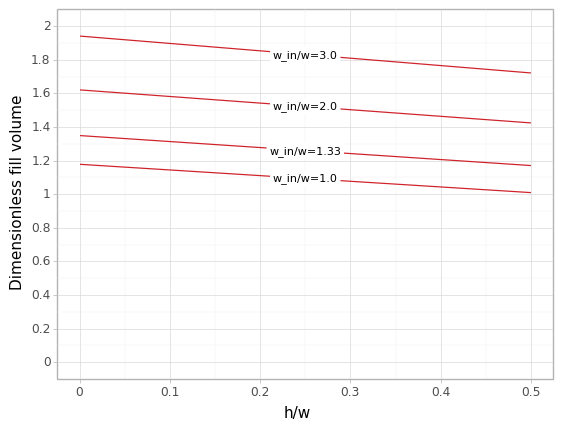
\includegraphics[width=\linewidth]{../figures/fig_2a.png}
    \caption{}
    \label{fig2a}
  \end{subfigure}
  \begin{subfigure}[b]{0.4\linewidth}
    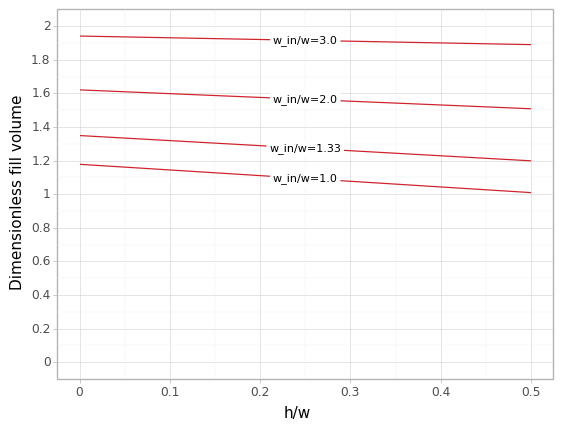
\includegraphics[width=\linewidth]{../figures/fig_2a_incorrect.png}
    \caption{}
    \label{fig2a_bad}
  \end{subfigure}
  \caption{Dimensionless fill volume, $\frac{V_{fill}}{hw^2}$ against $\frac{h}{w}$
  for four width ratios using a) the correct model, and b) an
  incorrect equation to replicate Figure O2a.}
\end{figure}

\subsubsection{Figure O2b}

The plot of squeezing coefficient (Figure \ref{fig2b}) replicates Figure O2b.

\begin{figure}[ht]
  \centering
  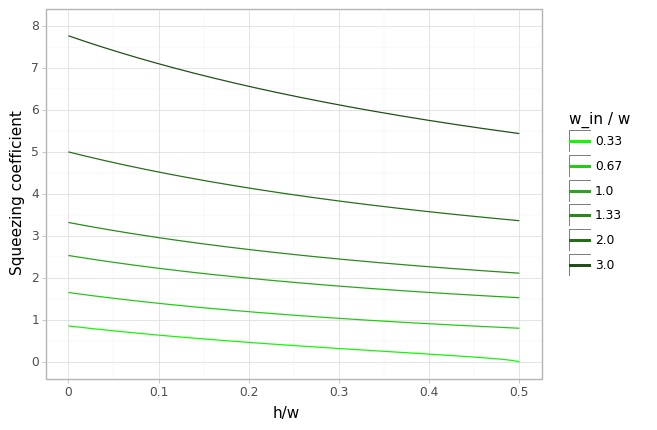
\includegraphics[width=0.8\linewidth]{../figures/fig_2b.png}
  \caption{Squeezing coefficient, $\alpha$ against height / channel width
  for six width ratios. Replication of Figure O2b.}
  \label{fig2b}
\end{figure}

\subsubsection{Figure O3}

The figure of total fill volume (Figure \ref{fig3}) very closely replicates Figure O3, with a small
difference. For all lines corresponding to gas bubbles (solid lines), the replicated figure appears to be
an exact match. However, for the single line corresponding to the liquid-liquid droplets (dashed line), the
slope is steeper than in our figure.

\begin{figure}[ht]
  \centering
  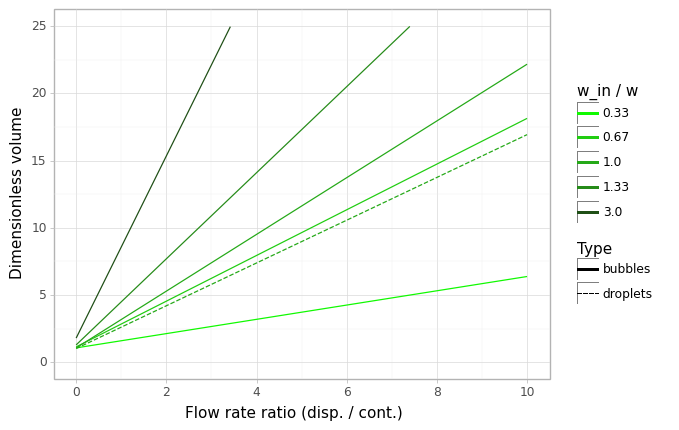
\includegraphics[width=0.8\linewidth]{../figures/fig_3.png}
  \caption{Total dimensionless volume, $\frac{V}{hw^2}$ against flow rate ratio $\frac{q_d}{q_c}$
  for various width ratios and dispersed fluid types. Gas bubbles are shown with solid lines, liquid-liquid droplets
  shown with dashed line. Replication of Figure O3.}
  \label{fig3}
\end{figure}

\subsubsection{Figure O6}

The figure depicting the evolution of the receding interface (Figure \ref{fig6}) replicates
the corresponding Figure O6 well.

\begin{figure}[!htb]
  \centering
  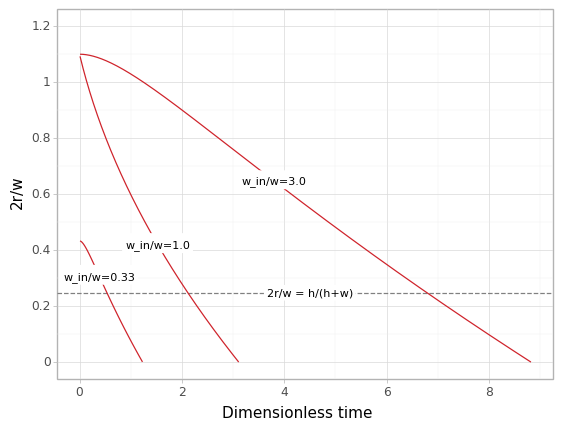
\includegraphics[width=0.8\linewidth]{../figures/fig_6.png}
  \caption{Evolution of the receding interface as $\frac{2r}{w}$ against dimensionless time,
  $\frac{q_c}{hw^2}t$ for various width ratios. Dashed line shows $\frac{2r_{pinch}}{w}=\frac{h}{h+w}$,
  the threshold at which the model predicts pinch off to occur.
  Replication of Figure O6.}
  \label{fig6}
\end{figure}

\section{Discussion}

\subsection{Model replication}

Python modules were developed that successfully replicate the model in the original work.
These modules have strong code testing coverage, and adhere to Python community guidelines.
Model logic was organized into modules to keep it separate from the specific geometries
used to replicate the figures. By doing so, it is easier to test the functions constituting
the model and makes it easy to reuse the code for generalization. All module functions can be
imported into any Python program and used for prediction.

\subsection{Replication of figures}

All figures could be replicated, although with one discrepancy in our figure corresponding to 
Figure O3.

Given that the same functions from the modules are used to calculate dimensionless volume for both
liquid-liquid droplets and air bubbles, and that the air bubble results match theirs, it is
unlikely that the modules are incorrect. This means that one or more of the provided geometries
are different in our implementation and theirs.

Since the liquid-liquid droplet line appears to be labeled
as $\frac{w_{in}}{w}=0.67$ though the figure caption states $\frac{w_{in}}{w}=1.0$, we considered that
perhaps the true ratio was $0.67$. However, reducing this ratio only reduces the slope,
exacerbating the discrepancy.

Notably, it appears that the experimental results plotted in Figure O3
more closely match the line for liquid-liquid droplets in our Figure \ref{fig3}
than theirs. This may be an indication that when generating model results, they incorrectly
entered one or more geometric parameter.

\subsection{Challenges}

Developing verbose geometry-based functions in the filling module was slightly difficult to do.
The original work gives some explanation of how the equations were derived, but many steps were
omitted. This is understandable since describing in full detail would result in extremely long
exposition. For the same reason, the geometric calculations performed in our modules
are even more low-level than described here.

While replication could have been done by simply using the simplified equation, having
the geometry-based code provided assurance that our model implementation was correct since
we could test the results of the verbose code against the simplified equation. This became very
useful when exact replication of Figure O2a was elusive.

Exact replication of Figure O2a was a matter of luck. When our initial implementation of the
model equations did not match the original figure, we resorted to implementing the simplified
equation in several programming languages, assuming we had made some mistake despite the
verbose code matching our implementation of the simplified equation. It is fortunate that we
happened to eventually make what we believe is the same mistake as the original authors one of
those times, allowing us to replicate their figure.

The fact that eventually we, and likely the original authors, made mistakes in entering that equation
demonstrates how easy it is to make mistakes that can greatly affect results when writing code.
This illustrates the practical utility of software tests. Unit testing makes it far more likely that
such bugs will be caught in development.

Perhaps the greatest challenge to replicating the original results came from their
omission of an explicit equation providing $2r$ as a function of time $t$, which must have been
used to generate Figure O6. Further, the authors did not indicate which equations could be used to
derive such a relationship. It was with a fair amount of effort that the relationship
was derived for this replication.

\section{Conclusion}

The model in the original work could be fully replicated based solely on the contents of
that article. However, two discrepancies in the figures were encountered upon replication.
The first was likely due to a mistake in the original code; the original figure was successfully
replicated in this work by deliberately using an equation that was incorrect.
Although the second discrepancy remains, it is likely due to differences
in the geometries provided to generate the original figure and those presented in the figure caption.
This notion is supported by the closer alignment of their experimental results to our modeling results
than theirs.

\section{Code availability}

All source code is available at \url{https://github.com/schackartk/t-junction_model_replication}

\section{Author contributions}

We report author contributions according to the CRediT taxonomy\supercite{allen_how_2019}.

\noindent KS: Conceptualization, Formal Analysis, Investigation, Methodology,
Project Administration, Software, Validation, Visualization, Writing — original draft,
Writing — review \& editing;

\noindent KK: Conceptualization, Investigation, Validation, Writing — original draft,
Writing — review \& editing

\section{Funding}

The authors received no financial support for the research, authorship,
and/or publication of this article.

\section{Acknowledgements}

The authors would like to thank Dr. Qiudong Wang at the University of Arizona for
challenging KS to replicate the results of a math modeling paper as a final project, and
for providing feedback on the first iteration of this project (originally written
in MATLAB, available at \url{https://github.com/schackartk/MATH585}).

\section{Conflict of interest}

The authors declare that the research was conducted in the absence of any commercial or
financial relationships that could be construed as a potential conflict of interest.
